\newpage
\section{Durchführung}
\subsection{Messschaltung}
Die Ladungen $Q$, die sich am Anodendraht sammeln fließen über einen
Wiederstand $R$ ab und werden über einen Spannungsimpuls über einen Kondensator $C$
ausgekoppelt, über einen Verstärker vergrößert und somit vom Zählgerät regristriert.
\begin{figure}
    \centering
    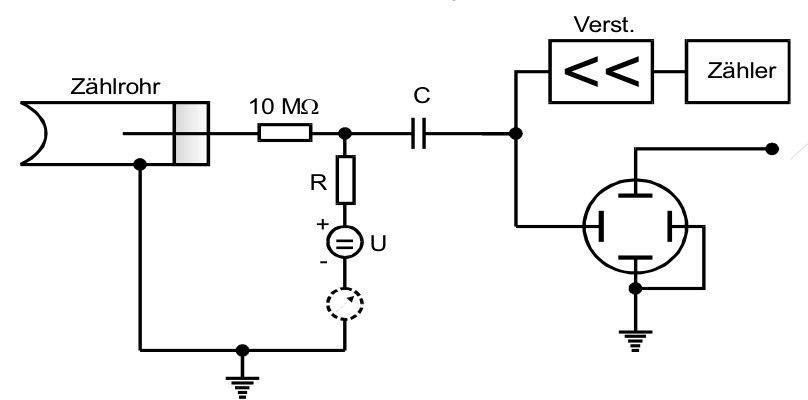
\includegraphics[width=0.7\textwidth]{input/messapperatur.jpg}
    \caption{Darstellung der Messapperatur mit dem Zählrohr und der Schaltung
    von Widerstand, Kondensator, Verstärker und Zähler.\cite[226]{anleitung}}
\end{figure}

\subsection{Aufnahme der Charakteristik}
Gemessen wird die Zählrate einer $\beta$-Quelle in Abhängigkeit der Betriebsspannung $U$.
$U \leq 700\si{V}$ sollte dabei eingehalten werden, um das Zählrohr durch
einen zuhohen Intensitätsstrom nicht zu zerstören. Zudem übersteigt die Impulsrate nicht $100\;/\;\si{s}$
damit die Totzeit-Korrektur vermieden werden kann.\\
Gemessen wir hierfür die Anzahl der Zerfälle pro Zeitintervall in Schritten von $\Delta U=10\si{V}$.
\subsection{Bestimmung der Totzeit}
Für die Bestimmung der Totzeit können zwei Methoden genutzt werden.
\subsubsection*{Oszilloskop}
Durch Ablesen der ersten beiden Peaks am Oszilloskop, welche die Spannungsimpulse graphisch visualisiert,
kann die Totzeit direkt bestimmt werden.
\subsubsection*{Zwei-Quellen-Methode}
Mit einer zusätzlichen $^{204}Tl$-Quelle die näher an das Geiger-Müller Zählrohr gerückt ist,
lässt sich über Gl. \ref{eqn:2Quellen} mit den gemessenen Zählraten die Totzeit $T$ berechnen.
\subsection{Bestimmung des Zählrohrstroms}
Mithilfe Gl. \ref{eqn:strom} kann aus dem mittleren Zählstrom $I$
die freigesetzten Ladungen pro eingefallendem Teilchen berechnet werden. 
\label{sec:Durchfuehrung}
